\documentclass[12pt]{article}
\usepackage[left=15mm,top=0.5in,bottom=0.5in,centering]{geometry}
\usepackage{listings}
\usepackage{framed}
\usepackage{graphicx}
\usepackage{wrapfig}
\usepackage{floatrow}
\usepackage{subfigure}
\usepackage{color}
\usepackage{amsmath}
\usepackage{lipsum}
\usepackage{hyperref}
\usepackage{amssymb}
\usepackage{rotating}
\usepackage{tikz}
\usepackage{tabu}
\usepackage{titlesec}
%\usepackage{algorithm}
\usepackage[linesnumbered,ruled,vlined,english,onelanguage]{algorithm2e}
%\usepackage{algorithmic}
\usepackage[noend]{algpseudocode}
\definecolor{dkgreen}{rgb}{0,0.6,0}
\definecolor{gray}{rgb}{0.5,0.5,0.5}
\definecolor{mauve}{rgb}{0.58,0,0.82}
\lstset{frame=tb,
	language=Java,
	aboveskip=3mm,
	belowskip=3mm,
	showstringspaces=false,
	columns=flexible,
	basicstyle={\small\ttfamily},
	numbers=none,
	numberstyle=\tiny\color{gray},
	keywordstyle=\color{blue},
	commentstyle=\color{dkgreen},
	stringstyle=\color{mauve},
	breaklines=true,
	breakatwhitespace=true,
	tabsize=3
}
\newcounter{question}
\setcounter{question}{0}
\def\thequestion{{\bf{Question \arabic{question}. }}\space }
\newcommand{\Question}[1]{\pagebreak \stepcounter{question}\noindent\thequestion#1\par}
\newcounter{countpart}[question]
\setcounter{countpart}{0}
\def\thepart{\\ \par (\alph{countpart}) \space}
\newcommand{\Part}[1]{\stepcounter{countpart}\noindent\thepart#1\normalfont{}}
\newenvironment{Parts}{\par\medskip
	\noindent \rmfamily}{\medskip}

\def\BeginSolution{\begin{framed}\noindent \normalfont{}}
	\def\EndSolution{\end{framed}\pagebreak}
\newcommand{\mat}[1]{\mathbf{#1}}
\newcommand{\matG}[1]{\boldsymbol{#1}}
\newcommand{\bm}[1]{\boldsymbol{#1}}
\def\real{\mathbb{R}}
\def\R{\mathbb{R}}
\newcommand{\norm}[1]{\left\lVert#1\right\rVert}
%\newcommand*\EE[1]{\ensuremath{\text{\textsc{e}}#1}}
\def\EE{\mathbb{E}}
\def\ev{\mathbb{E}}
\def\P{\mathbf{P}}
\def\y{\vec{y}}
\def\X{\mathbf{X}}
\def\x{\vec{x}}
\def\w{\vec{w}}
\def\b{\vec{b}}
\def\r{\vec{r}}
\def\T{^{\top}}
\def\argmin{\text{arg}\min\limits}
\def\argmax{\text{arg}\max\limits}
\def\I{\mathbb{I}}
\def\A{\vec{A}}
\def\tran{^{\top}}
\def\W{\mathbf{W}}
\def\z{\mathbb{z}}
\def\ell{l}
\newcommand{\diag}{\mathop{\mathrm{diag}}}
\allowdisplaybreaks
\usepackage[final]{pdfpages}
\setboolean{@twoside}{false}
\setcounter{MaxMatrixCols}{20}

\begin{document}
	\title{CS294-112 HW1\vspace{-2ex}}
	\author{Huanjie Sheng, 25928718\vspace{-2ex}}
	\date{\today \vspace{-2ex}}
	\maketitle
	%\addcontentsline{toc}{subsection}{Appendices}
	%\renewcommand{\thesubsection}{(\alph{subsection})}
	%\titleformat*{\subsection}{\normalfont}
	
	\stepcounter{section}
	\section{Behavioral Cloning}
	\stepcounter{subsection}
	\subsection{Comparison between behavioral cloning and expert policy}
	
	\begin{tabu} to 1.0\textwidth {  |X[c] |X[c] |X[c] |X[c] |X[c] | }
		\hline
		& exp(mean) & exp(std) & bc(mean) & bc(std)\\
		\hline
		Ant-v2  & 4823.29695049 & 100.901786378 & 4825.32305121 & 113.912392909\\
		\hline
		
		Humanoid-v2  & 10401.0887849 & 41.1015403998 & 2219.26290071 & 1302.88074545\\
		\hline
		
	\end{tabu}\\ \\
	exp: expert; bc: behavioral cloning \\ \\
	We can see that behavioral cloning performs well in \textbf{\textit{Ant-v2}} but very badly in \textbf{\textit{Humanoid-v2}}.
	\\ \\
	\textbf{Here are the parameters I used for this simulation:}\\
	max\_timesteps: 1000, num\_rollouts: 20, epochs: 500 \\
	\\
	\textbf{Here are the policy architecture used:}\\
	hidden\_layers=2, layer\_size=64, activation\_func=tf.nn.relu 
	
	\subsection{Hyperparameter tuning in behavioral cloning}
	\begin{figure}[!htbp] 
		\floatbox[{\capbeside\thisfloatsetup{capbesideposition={right,top},capbesidewidth=0.5\textwidth}}]{figure}[\FBwidth]
		{\caption[caption]{
				Hyperparameter tuning of epochs with the same model as in 2.2.
				Here are the parameters I used:\\ \hspace{0.5\textwidth}
				expert\_policy\_file: ./experts/Humanoid-v2.pkl,\\ \hspace{0.5\textwidth}
				envname: Humanoid-v2,\\ \hspace{0.5\textwidth}
				max\_timesteps: 1000,\\ \hspace{0.5\textwidth}
				num\_rollouts: 20,\\ \hspace{0.5\textwidth}
				I chose epochs because it directly affects whether the training process converges.  Besides, it's easy to tune.
			}\label{fig:hyper}}
		{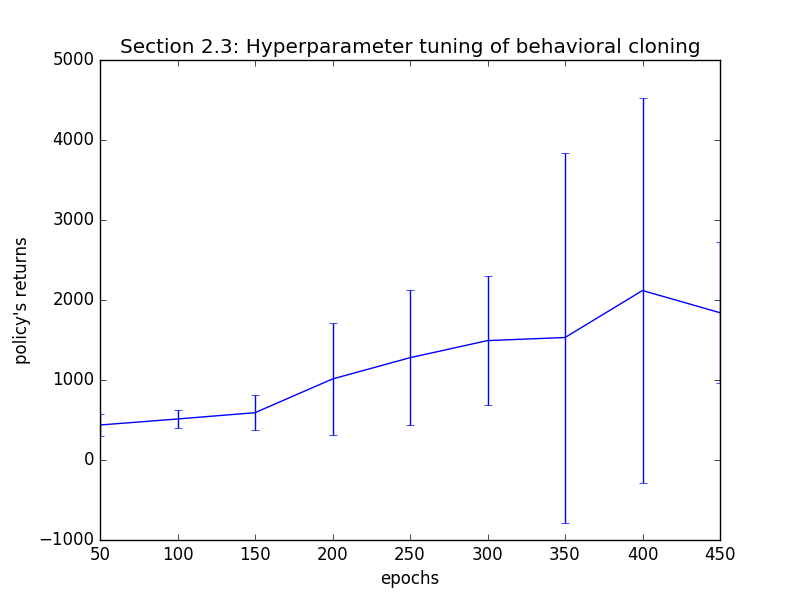
\includegraphics[width=0.5\textwidth]{section23.png}}
	\end{figure}
	\pagebreak
	
	\section{DAgger}
	\stepcounter{subsection}
	\subsection{Comparison between behavior cloning and expert policy}
	%\noindent \rule{\textwidth}{1pt}
	\begin{figure}[!htbp] 
		\floatbox[{\capbeside\thisfloatsetup{capbesideposition={right,top},capbesidewidth=0.5\textwidth}}]{figure}[\FBwidth]
		{\caption[caption]{
				I used the same neural network mode las in behavioral cloning with two hidden layers of 64 hidden nodes per layer, which use ReLU as activation functions.\\ \hspace{0.5\textwidth}
				Here are the parameters I used:\\ \hspace{0.5\textwidth}
				expert\_policy\_file: ./experts/Humanoid-v2.pkl,\\ \hspace{0.5\textwidth}
				envname: Humanoid-v2,\\ \hspace{0.5\textwidth}
				max\_timesteps: 1000,\\ \hspace{0.5\textwidth}
				num\_rollouts: 20,\\ \hspace{0.5\textwidth}
				epochs: 500,\\ \hspace{0.5\textwidth}
				dagger\_runs: 10, \\ \hspace{0.5\textwidth}
				It should be noted that "num\_rollouts" applies to both the expert demonstration and the correction for each dagger iteration.
			}\label{fig:dagger}}
		{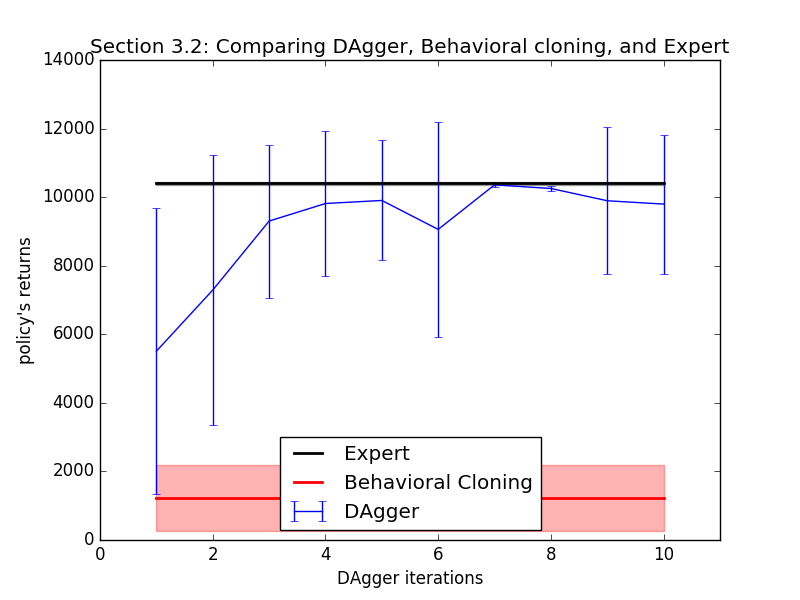
\includegraphics[width=0.5\textwidth]{section32.png}}
	\end{figure}
	
	\section{Policy architecture}
	\subsection{Policy architecture of behavioral cloning}
	\begin{tabu} to 1.0\textwidth {  |X[c] |X[c] |X[c] | }
		\hline
		& mean & std\\
		\hline
		expert  & 10410.3113272 & 34.5014719634\\
		\hline
		original  & 1627.43551917 & 1271.28443921\\
		\hline
		hidden\_layers=6  & 627.643695252 & 173.365926011\\
		\hline
		layer\_size=16  & 529.67947482 & 202.227319372\\
		\hline
		activation\_func=tt.nn.tanh  & 597.21387704 & 144.390361908\\
		\hline
	\end{tabu}\\ \\
	\begin{figure}[!htbp] 
		\floatbox[{\capbeside\thisfloatsetup{capbesideposition={right,top},capbesidewidth=0.5\textwidth}}]{figure}[\FBwidth]
		{\caption[caption]{
			From left to right: expert, original model, model with six hidden layers, model with 16 hidden nodes per layer, model using tanh as activation function.\\ \hspace{0.5\textwidth}
			Here are the parameters I used:\\ \hspace{0.5\textwidth}
			expert\_policy\_file: ./experts/Humanoid-v2.pkl,\\ \hspace{0.5\textwidth}
			envname: Humanoid-v2,\\ \hspace{0.5\textwidth}
			max\_timesteps: 1000,\\ \hspace{0.5\textwidth}
			num\_rollouts: 20,\\ \hspace{0.5\textwidth}
			epochs: 300,\\ \hspace{0.5\textwidth}
			All modification performs worse than my original model which is copied from the TensorFlow's tutorial.  More layers is worse probably because it overfits.  Less hidden nodes is worse probably because it underfits.  tanh is worse might be because I did not normalize the input data.
		}\label{fig:test}}
		{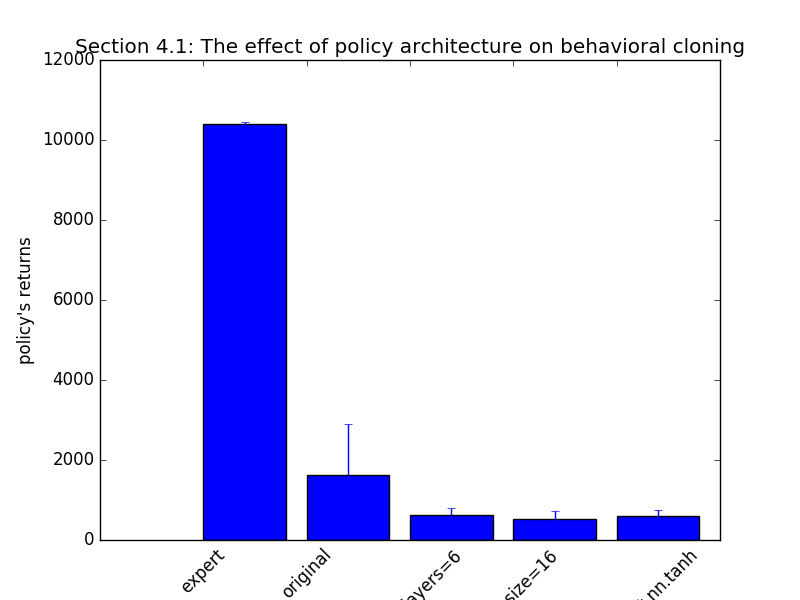
\includegraphics[width=0.5\textwidth]{section41.png}}
	\end{figure}
	
	
	
\end{document}